% =========================================================
%  Chapter 2 — The Einstein Model
%  Style: student-voice notes matching the personal style guide
% =========================================================
\section{The Einstein Model}

Now let's talk about why we need a new model and what it actually changes. We finished the classical model and established that it cannot describe amplification. We now need a different framework to describe the interaction between light and matter — one that can. We start with the \textbf{Einstein model}.

The two most fundamental changes from the classical picture are:
\begin{enumerate}
    \item \textbf{Matter is now described by discrete energy levels.} The material is no longer a continuous medium with a smoothly varying susceptibility. Instead, each atom (or, in a semiconductor, each electron-hole pair) exists at a specific energy level $E_i$, and transitions between levels are the only way energy is exchanged.
    \item \textbf{Light is now described by photons, not waves.} We are working fully in the quantum picture now. A photon carries energy $E = h\nu$ and interacts with the atom as a discrete packet of energy, not as a continuous oscillating field.
\end{enumerate}

\begin{figure}[H]
    \centering
    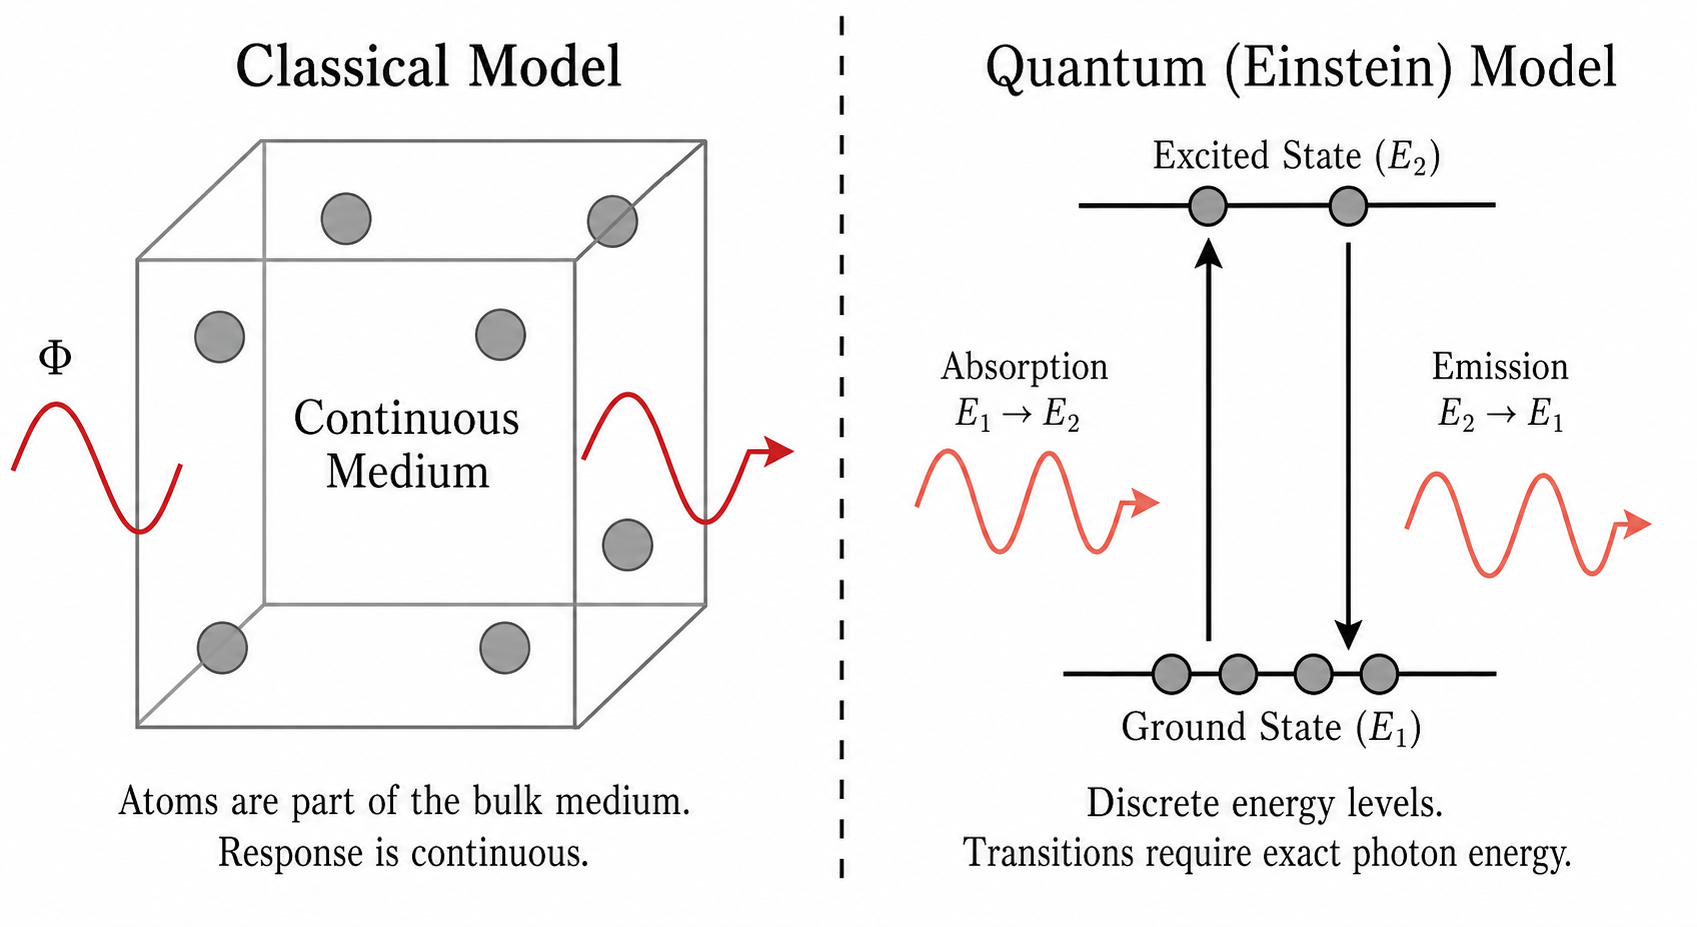
\includegraphics[width=0.6\textwidth]{Figures/Chapter 2/classical_vs_quantum_medium.jpg}
    \caption{Classical vs. Quantum Material: The classical continuous medium compared to the discrete quantum energy states of the Einstein model.}
    
\end{figure}

\begin{motivation}[Why the Einstein Model Works Where the Classical One Fails]
The classical model built a powerful toolkit — susceptibility, complex refractive index, line shape, absorption cross section — but ran into a hard wall: every factor in $\alpha$ is strictly positive, making optical amplification physically impossible. The Einstein model breaks this wall by replacing the continuous medium with a material governed by \textbf{discrete quantum energy levels}. Instead of a driven spring, we now picture a two-level atom with a ground state $E_1$ and an excited state $E_2$. The critical insight is that the population balance between $N_1$ and $N_2$ will control the sign of gain — and by artificially inverting that balance ($N_2 > N_1$, population inversion), we will finally achieve amplification.
\end{motivation}

\subsection{Energy Level Populations}

In the Einstein model, each energy level $E_i$ is characterised by a number $N_i$ — the \textbf{atom density} (or \textbf{population density}) of that level, defined as the number of atoms per unit volume currently occupying it. Note that this is different from the classical picture: in the classical model we had a single quantity $N_A$ representing the total number of atoms per unit volume for the entire material. Here, $N_A$ is split — each energy level has its own population $N_i$, and the total number of atoms is $N_A = \sum_i N_i$.

We will work with a \textbf{two-level system}, which is the simplest non-trivial case. We have:
\begin{itemize}
    \item $E_1$, $N_1$: the lower energy level and its population.
    \item $E_2$, $N_2$: the upper energy level and its population, with $E_2 > E_1$.
\end{itemize}

\begin{figure}[H]
    \centering
    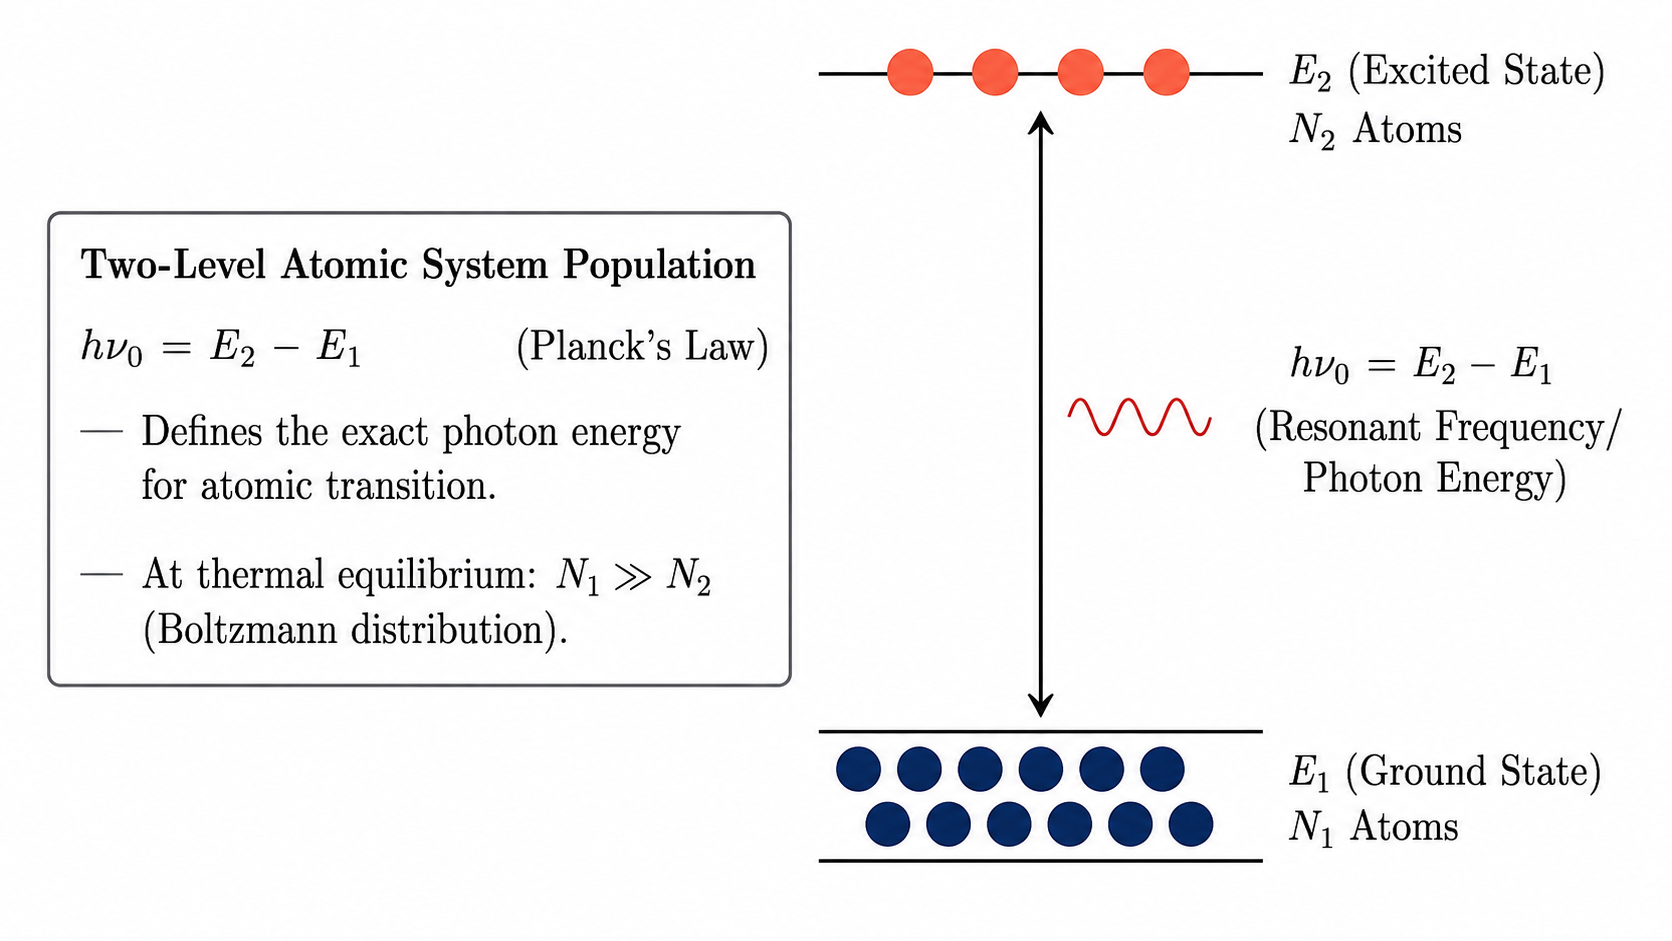
\includegraphics[width=0.6\textwidth]{Figures/Chapter 2/two_level_system.jpg}
    \caption{The Two-Level System: Depicting the lower and upper energy levels ($E_1$ and $E_2$), their respective populations ($N_1$ and $N_2$), and the required transition photon energy.}
    
\end{figure}

The energy difference between the two levels determines the photon frequency at which the atom can interact with light:
\begin{keyresult}
\begin{equation}
    E_{\text{photon}} = E_2 - E_1 = h\nu_0
\end{equation}
\end{keyresult}
where:
\begin{itemize}
    \item $h$: Planck's constant.
    \item $\nu_0$: the central transition frequency.
\end{itemize}

\subsection{A Brief Note on Semiconductors vs.\ Gases}

We need to be careful about the physical picture depending on the material:

\begin{enumerate}
    \item In a \textbf{semiconductor}: the entities that move between energy levels are \emph{electrons}. An electron in the valence band can absorb a photon and jump to the conduction band. The valence band is mostly full of electrons (many electrons, few holes), while the conduction band is mostly empty (few electrons, many holes). Because there are vacant states in the conduction band, electrons from the valence band can be promoted into them.
    \item In a \textbf{gas}: the entities that move are entire \emph{atoms}, transitioning from one energy level to another. The atom as a whole absorbs or emits a photon and changes its internal energy state.
\end{enumerate}

Since we are applying the Einstein model to gases first (as we said), whenever we say ``an atom moves from $E_1$ to $E_2$,'' we mean the atom's internal energy state changes — not that the atom physically moves in space.

\subsection{The Direct vs.\ Indirect Band Gap — A Brief Clarification}

Before continuing, let us note one important distinction for semiconductors that will matter later. In a \textbf{direct band gap semiconductor}, an electron and a hole undergoing recombination have the same momentum (the same wave vector $k$), meaning they sit directly above one another in the $E$-$k$ diagram. When they recombine, all the energy difference goes into a photon — this is efficient optical emission.

In an \textbf{indirect band gap semiconductor}, the electron and hole do not have the same momentum. Before they can recombine, the momentum mismatch must first be resolved — this happens by emitting a \textbf{phonon} (a quantised lattice vibration that carries the excess momentum). Only after the momentum is equalised can the energy difference be released as a photon. This extra phonon step makes indirect-gap semiconductors far less efficient light emitters, which is why materials like Silicon (indirect gap) are not used for lasers while Gallium Arsenide (direct gap) is.

\begin{figure}[H]
    \centering
    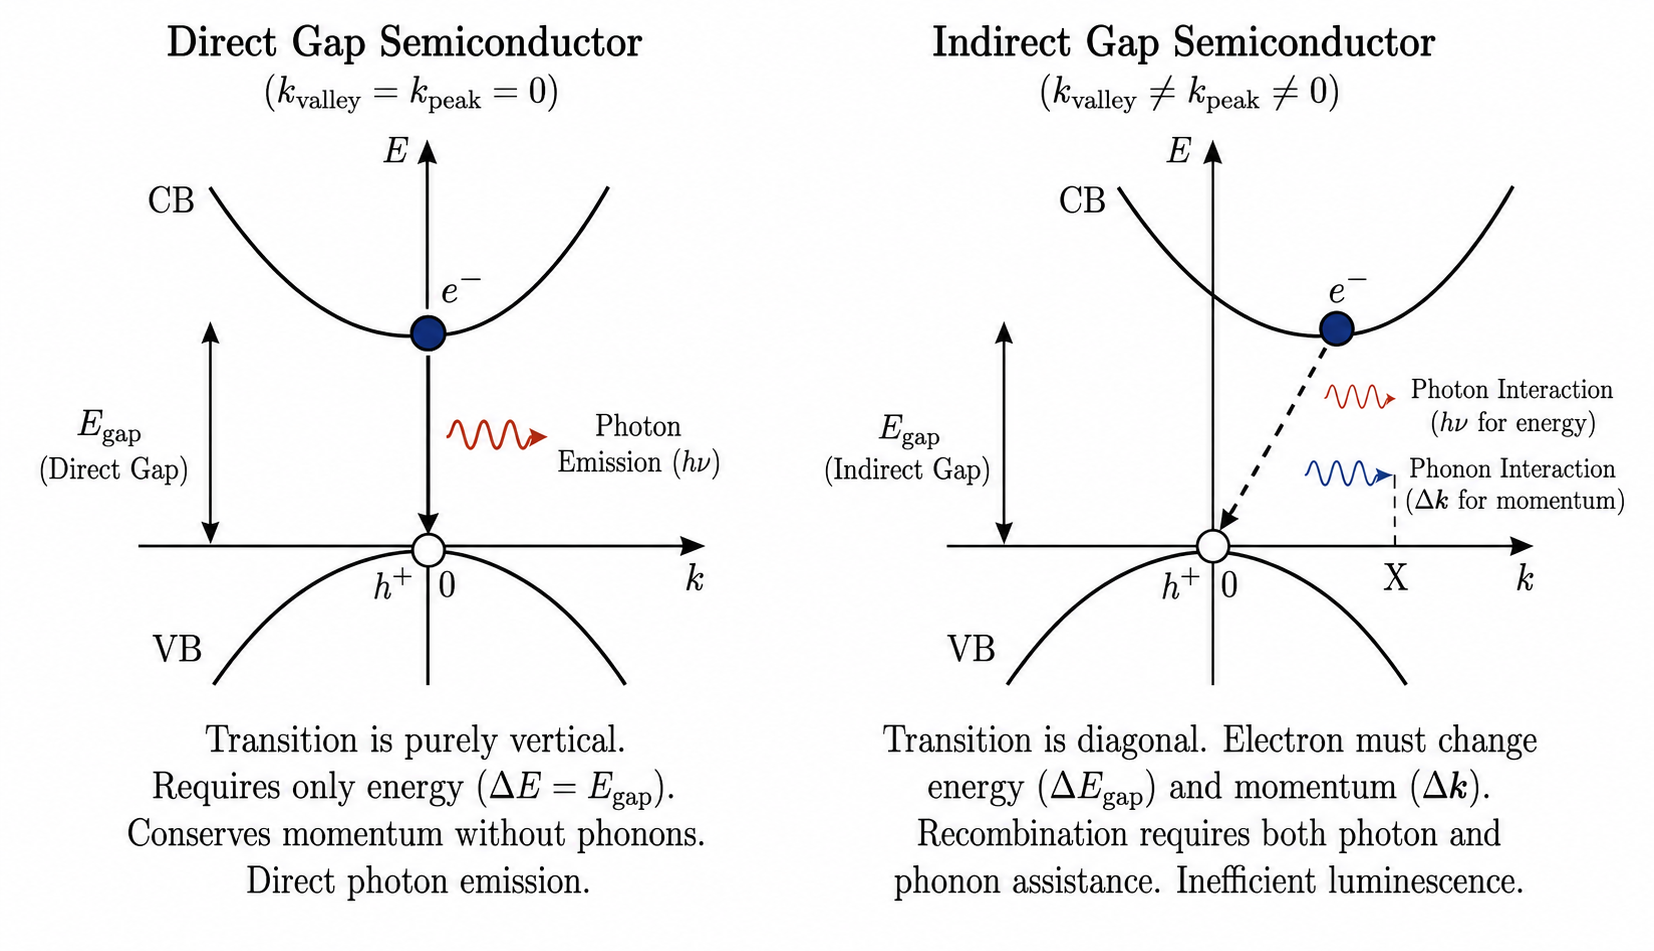
\includegraphics[width=0.6\textwidth]{Figures/Chapter 2/direct_vs_indirect_bandgap.jpg}
    \caption{Direct vs. Indirect Band Gap: Comparing the purely vertical transition of a direct gap emitter to the phonon-assisted diagonal transition of an indirect gap emitter.}
    
\end{figure}

Now, let's return to the main thread and look at the three fundamental processes by which atoms in the Einstein model interact with light.

\section{The Three Fundamental Processes}

In the Einstein model, the interaction between light and a two-level material can be described by \textbf{exactly three processes}. All three are probabilistic — none of them is certain to happen, but each has a well-defined rate. We study them one by one.

\subsection{Process 1: Spontaneous Emission}

Suppose an atom is sitting in the upper energy level $E_2$. This is not its natural, preferred state — the atom's ground state is $E_1$. Regardless of how it got to $E_2$ (we don't care about the past), the atom will inherently try to shed the extra energy and relax back down to $E_1$. It does so by emitting a photon whose energy is exactly equal to the difference between the two states:
\begin{equation*}
    E_{\text{photon}} = E_2 - E_1 = h\nu_0
\end{equation*}

This process is called \textbf{spontaneous emission} because it happens entirely on the atom's own initiative. There is no external trigger, no applied field, and no incident photon required; the atom simply falls from $E_2$ to $E_1$ on its own and a photon pops out.

Critically, the photon produced by spontaneous emission has a completely \textbf{random direction, random polarisation, and random phase}. It is essentially noise from the perspective of building a coherent beam. However — and this is a point to keep in the back of your mind — spontaneous emission is the \emph{seed} that starts laser action, even though the laser itself runs on stimulated emission. We will understand exactly why when we get to the laser structure. For now, just note this fact.

\begin{figure}[H]
    \centering
    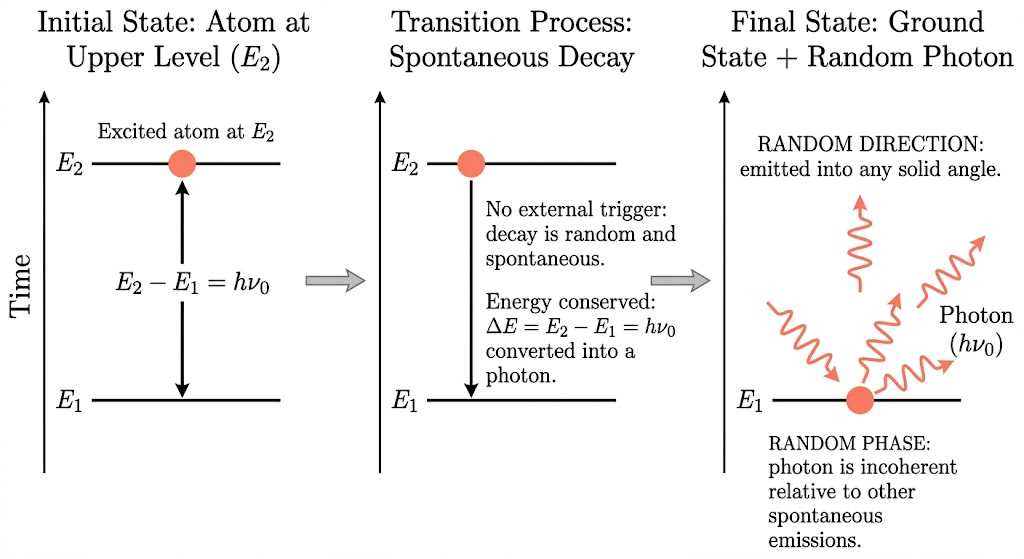
\includegraphics[width=0.7\textwidth]{Figures/Chapter 2/spontaneous_emission.jpg}
    \caption{Spontaneous Emission: An atom in the excited state ($E_2$) decays spontaneously to the ground state ($E_1$), emitting a photon with random phase and direction.}
    
\end{figure}

To describe this process mathematically, we track the rate of change of the upper-level population $N_2$ with time. Since spontaneous emission removes atoms \emph{from} $E_2$, it causes $N_2$ to decrease. Now, how fast does this depletion happen? We characterise each atom's tendency to decay by the \textbf{spontaneous emission lifetime} $\tau_{sp}$ — the \emph{average} time a single atom spends sitting in $E_2$ before it spontaneously falls down to $E_1$. If an atom \emph{on average} waits a time $\tau_{sp}$ before decaying, then the probability that it decays in any small time interval $dt$ is simply $dt/\tau_{sp}$. In other words, the \textbf{decay probability per unit time for a single atom} is the \textbf{Einstein A coefficient} ($A = 1/\tau_{sp}$). We have $N_2$ atoms per unit volume all independently undergoing this same process, so the total rate at which the $E_2$ population decreases is just this per-atom rate multiplied by the number of atoms available:

\begin{equation*}
    \left.\frac{dN_2}{dt}\right|_{sp} = -A\,N_2
\end{equation*}

where $N_2$ is the population density of $E_2$ (atoms per unit volume), $A$ has units of $\text{s}^{-1}$, and the negative sign reflects that atoms are \emph{leaving} $E_2$.

\subsection{Process 2: Absorption}

Absorption is the process by which an atom in its ground state $E_1$ absorbs an incoming photon and is promoted to the upper level $E_2$, but only if the photon's energy exactly matches the transition energy:
\begin{equation*}
    E_{\text{photon}} = E_2 - E_1 = h\nu_0
\end{equation*}

What happens to the atom after the absorption is irrelevant to this process — it might subsequently decay via spontaneous emission, lose energy through collisions, or undergo something else entirely. We describe absorption in isolation.

\begin{figure}[H]
    \centering
    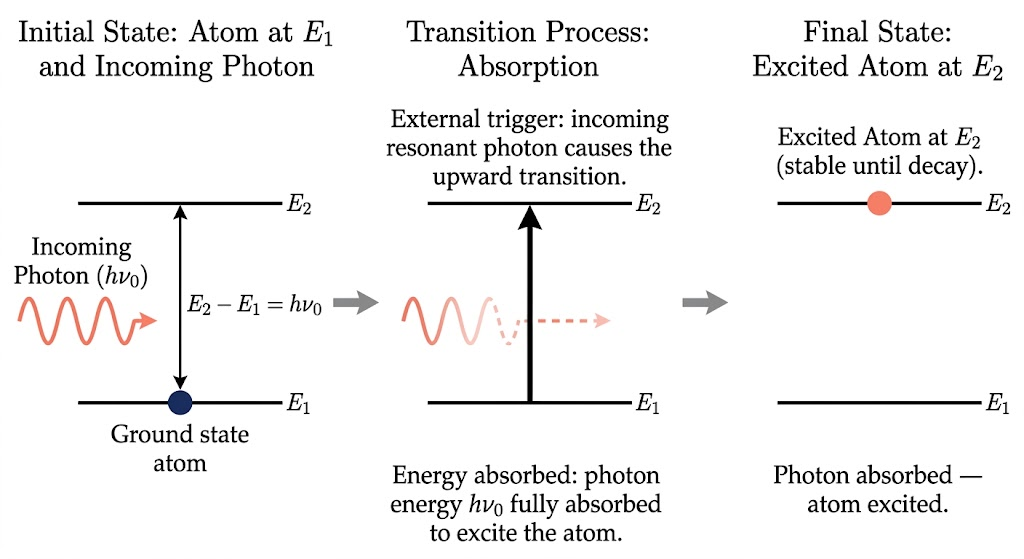
\includegraphics[width=0.7\textwidth]{Figures/Chapter 2/photon_absorption.jpg}
    \caption{Absorption: An incoming photon interacts with an atom in the ground state ($E_1$), transferring its energy to promote the atom to the excited state ($E_2$).}
    
\end{figure}

Mathematically, absorption takes atoms \emph{into} $E_2$ from $E_1$, increasing $N_2$. Unlike spontaneous emission, this process is not self-driven — it requires an incoming photon. The rate therefore depends on both how many atoms are sitting in $E_1$ available to absorb ($N_1$) and how dense the photon field is at the resonance frequency (the energy spectral density $\rho(\nu)$). We capture this through the \textbf{Einstein $B_{12}$ coefficient}, where the subscript ``12'' encodes the direction of the transition (from level 1 to level 2):

\begin{equation*}
    \left.\frac{dN_2}{dt}\right|_{abs} = B_{12}\,\rho(\nu)\,N_1
\end{equation*}

where:
\begin{itemize}
    \item $N_1$: the population density of $E_1$ (atoms per unit volume available to be excited).
    \item $B_{12}$: the absorption rate per atom per unit energy spectral density (units: $\text{m}^3/(\text{J}\cdot\text{s}^2)$).
    \item $\rho(\nu)$: the \textbf{energy spectral density} of the incident radiation — the energy stored per unit volume per unit frequency (units: $\text{J}/(\text{m}^3 \cdot \text{Hz})$).
\end{itemize}

\subsection{Process 3: Stimulated Emission}

Stimulated emission is the most interesting process, and the one that makes lasers possible. Here, an incoming photon interacts with an atom that is \emph{already sitting in the upper level $E_2$} (already in an excited state). The photon \emph{stimulates} the atom to fall down from $E_2$ to $E_1$, releasing its stored energy in the form of a \emph{second photon}.

The remarkable thing is the nature of the emitted photon: it is an \textbf{exact clone} of the incident photon. It has the same frequency, the same phase, the same polarisation, and the same direction of propagation. This is fundamentally different from spontaneous emission, where the emitted photon has a random direction and phase. Stimulated emission produces coherent, phase-locked copies of the incoming photon — this is the physical mechanism behind laser amplification.

\begin{figure}[H]
    \centering
    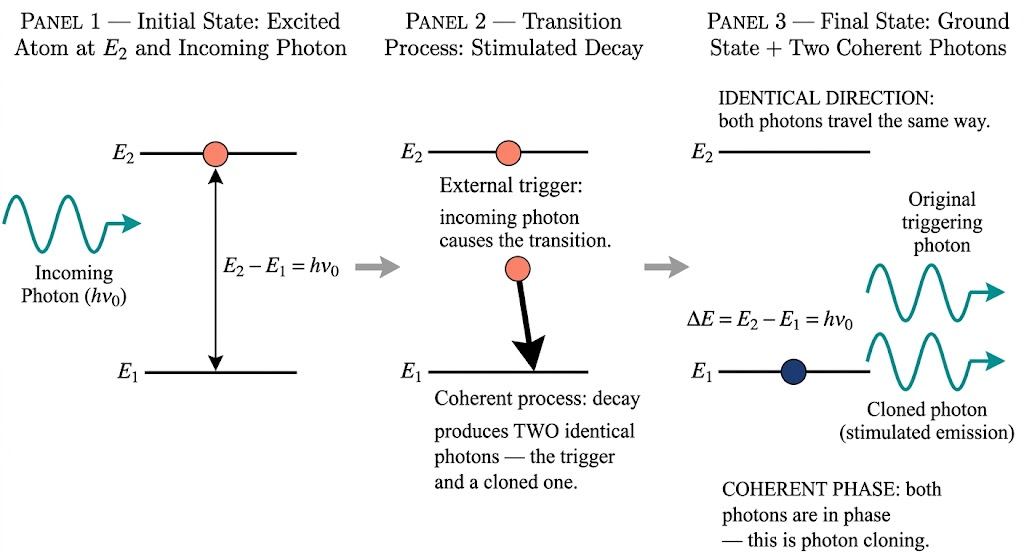
\includegraphics[width=0.7\textwidth]{Figures/Chapter 2/stimulated_emission.jpg}
    \caption{Stimulated Emission: An incoming photon triggers an excited atom ($E_2$) to decay. Crucially, the process yields two perfectly identical, coherent photons.}
    
\end{figure}


\begin{keyinsight}[Why the Emitted Photon is an Exact Clone]
Stimulated emission can be understood as the physical time-reverse of absorption. Maxwell's equations are time-reversal invariant — running an electromagnetic interaction backwards in time yields an equally valid physical process. Absorption takes \textbf{one photon in} and \textbf{zero photons out} (the photon is destroyed, the atom jumps up). Its time-reverse must therefore take \textbf{one photon in} and produce \textbf{two photons out}: the original triggering photon plus a newly emitted one. That two-photon output is precisely stimulated emission. This is why the emitted photon must be an exact clone of the incident one — time-reversal symmetry leaves no freedom to choose its frequency, phase, or direction independently.
\end{keyinsight}

To quantify this, the rate of stimulated emission must depend on the number of atoms available to be stimulated ($N_2$) and on the density of the incoming triggering photons ($\rho(\nu)$). We capture this through the \textbf{Einstein $B_{21}$ coefficient}, where the subscript ``21'' encodes the downward direction of the transition:

\begin{equation*}
    \left.\frac{dN_2}{dt}\right|_{stim} = -B_{21}\,\rho(\nu)\,N_2
\end{equation*}

where $B_{21}$ is the stimulated emission rate per atom per unit energy spectral density (same units as $B_{12}$).

\begin{keyinsight}[Three Processes and Their Signs]
It is worth pausing here to collect the signs and confirm they are all physically consistent. Spontaneous emission removes atoms from $E_2$ on its own ($-AN_2$). Absorption adds atoms to $E_2$ by taking them from $E_1$ ($+B_{12}\,\rho(\nu) N_1$). Stimulated emission removes atoms from $E_2$ with the help of an incident photon ($-B_{21}\,\rho(\nu) N_2$). All three are rates of change of $N_2$ and all three signs make physical sense.
\end{keyinsight}

\subsection{An Important Note on Probability}

None of these three processes is guaranteed to happen. Each one occurs with a certain probability. There are many other possible processes that can occur in a semiconductor or a gas — for example, an excited electron in the conduction band can give its extra energy to another electron already sitting in the conduction band (Auger process), or it can lose energy through phonon interactions. We acknowledge that these other processes exist. However, we study only the three processes above because they are the ones relevant to our goal of building a laser.

\section{Thermal Equilibrium and Deriving the Einstein Coefficients}

\subsection{Setting Up the Thermal Equilibrium Condition}

Now let's talk about thermal equilibrium. A material is said to be at \textbf{thermal equilibrium} when the population of each energy level stays constant in time — atoms may continuously transition up and down, but the net number in each level does not change. In semiconductor language, this is equivalent to saying that the generation rate equals the recombination rate everywhere.

Mathematically, thermal equilibrium means:
\begin{equation*}
    \frac{dN_2}{dt} = 0
\end{equation*}

The total rate of change of $N_2$ is the sum of contributions from all three processes:
\begin{equation*}
    \frac{dN_2}{dt} = \left.\frac{dN_2}{dt}\right|_{sp} + \left.\frac{dN_2}{dt}\right|_{abs} + \left.\frac{dN_2}{dt}\right|_{stim} = 0
\end{equation*}

Substituting the expressions we derived for each process:
\begin{equation*}
    -A\,N_2 + B_{12}\,\rho(\nu)\,N_1 - B_{21}\,\rho(\nu)\,N_2 = 0
\end{equation*}

Collecting the $\rho(\nu)$ terms on one side:
\begin{equation*}
    \rho(\nu)\left[B_{12}\,N_1 - B_{21}\,N_2\right] = A\,N_2
\end{equation*}

Solving for $\rho(\nu)$:
\begin{equation}
    \rho(\nu) = \frac{A\,N_2}{B_{12}\,N_1 - B_{21}\,N_2}
\end{equation}

The physical takeaway is that thermal equilibrium requires the spontaneous and stimulated downward flows to perfectly balance the upward absorption flow. Setting this balance yields our exact expression for the necessary equilibrium photon field $\rho(\nu)$.

This gives us $\rho(\nu)$ as a function of the populations and the Einstein coefficients. But we don't know the values of $B_{12}$ and $B_{21}$ yet, and we don't know the ratio $N_1/N_2$ in equilibrium without additional physics. We now bring in two separate pieces of known physics to evaluate both.

\subsection{The Boltzmann Population Ratio}

For gases and \textbf{non-degenerate semiconductors} (where the Fermi level sits safely inside the bandgap, at least $3k_BT$ away from the nearest band edge), particles at thermal equilibrium follow the \textbf{Boltzmann distribution}. The probability of finding an atom or electron at energy $E$ is proportional to $e^{-E/(k_B T)}$, where $k_B$ is Boltzmann's constant and $T$ is the absolute temperature. We explicitly assume the non-degenerate case to rule out \textbf{degenerate semiconductors} — heavily doped materials where the Fermi level is pushed into the bands, rendering them quasimetallic and strictly requiring Fermi-Dirac statistics instead.

For our two-level system, the population densities are proportional to these probabilities:
\begin{equation*}
    N_1 \propto e^{-E_1/(k_B T)}, \qquad N_2 \propto e^{-E_2/(k_B T)}
\end{equation*}

Taking their ratio:
\begin{equation*}
    \frac{N_1}{N_2} = \frac{e^{-E_1/(k_B T)}}{e^{-E_2/(k_B T)}} = e^{-(E_1 - E_2)/(k_B T)} = e^{(E_2 - E_1)/(k_B T)}
\end{equation*}

Since $E_2 - E_1 = h\nu_0$:
\begin{equation*}
    \frac{N_1}{N_2} = e^{h\nu_0/(k_B T)}
\end{equation*}

\begin{keyinsight}[The Iron Rule of Thermal Equilibrium]
Because the photon energy $h\nu_0$ and thermal energy $k_B T$ are strictly positive, the exponent $h\nu_0/k_B T$ is always strictly positive. Therefore, the ratio $e^{h\nu_0/k_B T}$ is always strictly greater than 1. This mathematically guarantees that $\mathbf{N_1 > N_2}$ without exception — thermal equilibrium inherently forbids population inversion ($N_2 > N_1$). For typical optical frequencies ($h\nu_0 \approx 1{-}3\,\text{eV}$) at room temperature ($k_B T \approx 26\,\text{meV}$), this exponent is huge, making the population ratio $N_1/N_2$ astronomically large. The statistical reality establishes a brutal baseline: matter exponentially crowds the lowest available energy state ($N_1 \gg N_2$), leaving the upper level virtually empty. Overcoming this natural limit is the fundamental hurdle in building a laser.
\end{keyinsight}

\begin{figure}[H]
    \centering
    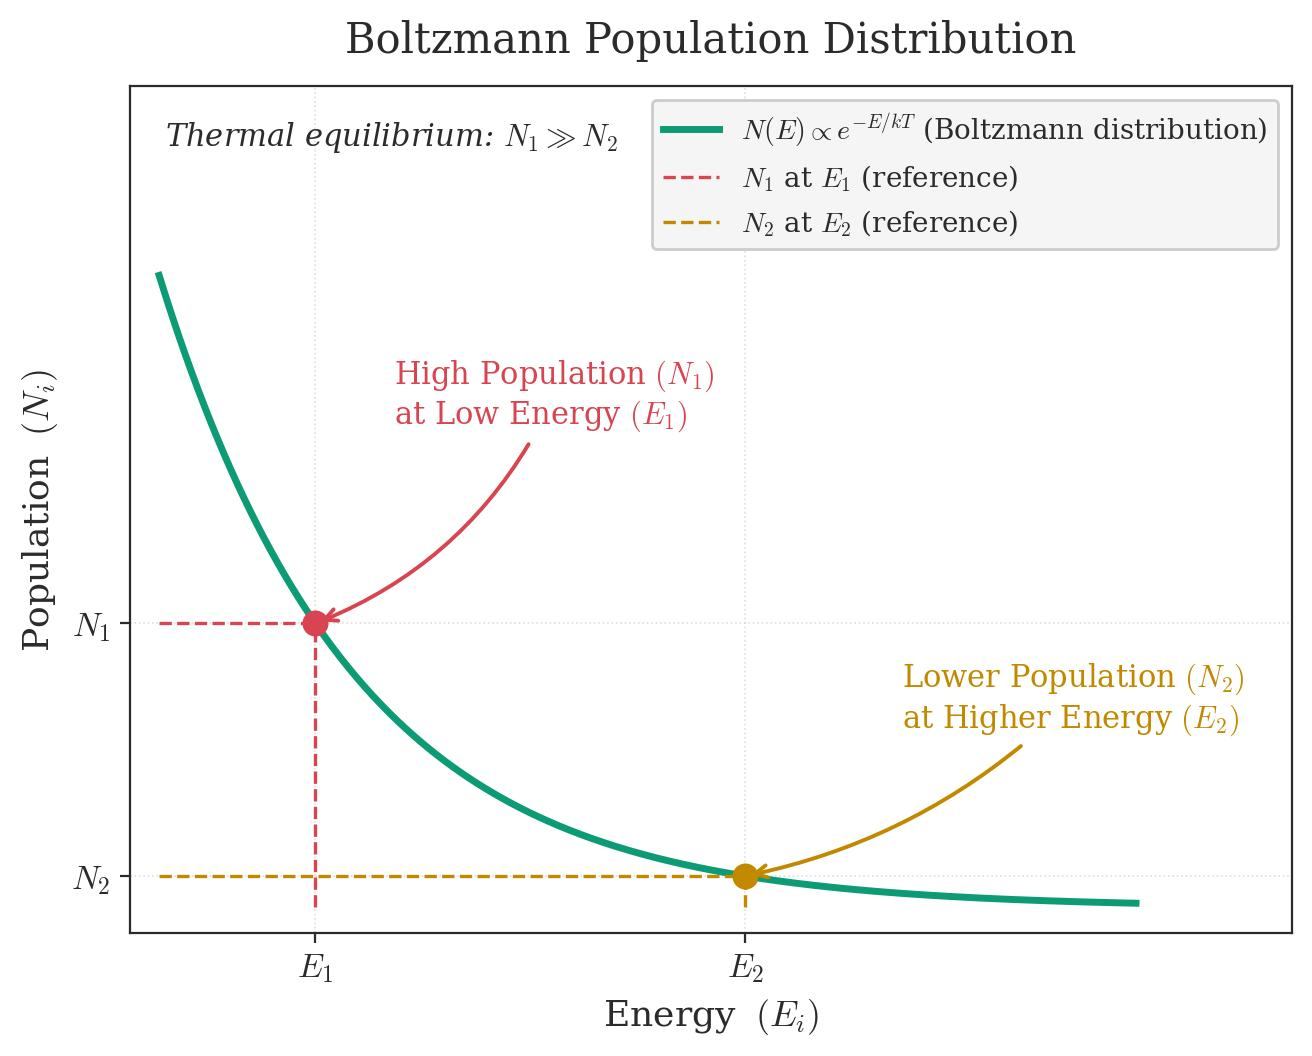
\includegraphics[width=0.65\textwidth]{Figures/Chapter 2/boltzmann_distribution.jpg}
    \caption{Boltzmann Population Distribution: The exponential decay curve illustrates why the lower energy state inherently sustains a vastly larger population than the upper state in thermal equilibrium.}
    
\end{figure}

\subsection{Substituting the Boltzmann Ratio into \texorpdfstring{$\rho(\nu)$}{E(nu)}}

We now substitute the explicit Boltzmann ratio into the preliminary $\rho(\nu)$ expression. Start from the required equilibrium photon field at resonance:
\begin{equation*}
    \rho(\nu) = \frac{A\,N_2}{B_{12}\,N_1 - B_{21}\,N_2}
\end{equation*}

Divide numerator and denominator by $N_2$:
\begin{equation*}
    \rho(\nu) = \frac{A}{B_{12}\,\dfrac{N_1}{N_2} - B_{21}}
\end{equation*}

We previously found that $\dfrac{N_1}{N_2} = e^{h\nu_0/(k_BT)}$. We substitute this absolute ratio into the denominator explicitly:
\begin{equation*}
    \rho(\nu) = \frac{A}{B_{12}\,e^{h\nu_0/(k_BT)} - B_{21}}
\end{equation*}

This is the energy spectral density implied by the Einstein model at thermal equilibrium. At this point we can see that we still have two unknowns: $B_{12}$ and $B_{21}$ (and we know $A = 1/\tau_{sp}$, but $\tau_{sp}$ itself depends on the atomic system). We need another equation. We get it by comparing with a known result.

\subsection{Comparing with Black-Body Radiation}

To solve for the unknowns, we imagine our two-level atoms sitting inside a completely sealed, heated cavity. The walls of this cavity perfectly absorb and emit radiation to maintain thermal equilibrium, filling the empty space inside with a dense field of photons known as \textbf{black-body radiation}. The spectrum of this radiation—exactly how much light energy is glowing at each frequency—depends entirely on the temperature $T$ of the cavity and nothing else.

The \textbf{energy spectral density of black-body radiation} is a continuous function of frequency $\nu$, yielding the well-known result from physics:
\begin{equation*}
     \rho_{BB}(\nu) = \frac{8\pi h\nu^3}{c^3} \cdot \frac{1}{e^{h\nu/(k_BT)} - 1}
\end{equation*}

This formula describes the energy distribution of radiation in a cavity at thermal equilibrium — which is exactly the same physical situation we have been computing with the Einstein model. Therefore, our derived equilibrium energy density $\rho(\nu)$ for the transition must perfectly match the thermal black-body spectrum at the specific resonance frequency $\nu_0$. Equating $\rho(\nu_0) =  \rho_{BB}(\nu_0)$ yields:
\begin{equation*}
    \frac{A}{B_{12}\,e^{h\nu_0/(k_BT)} - B_{21}} = \frac{8\pi h\nu_0^3}{c^3} \cdot \frac{1}{e^{h\nu_0/(k_BT)} - 1}
\end{equation*}

For this equality to hold at any arbitrary temperature $T$, the temperature-dependent terms on both sides must be functionally identical. We can see this clearly if we factor out $B_{12}$ from the denominator on the left side:
\begin{equation*}
    \frac{A}{B_{12}\left(e^{h\nu_0/(k_BT)} - \frac{B_{21}}{B_{12}}\right)} = \frac{8\pi h\nu_0^3}{c^3} \cdot \frac{1}{e^{h\nu_0/(k_BT)} - 1}
\end{equation*}

Comparing the denominators, this immediately requires that the ratio $B_{21}/B_{12} = 1$, or simply:
\begin{equation*}
    B_{12} = B_{21} \equiv B
\end{equation*}

This is a remarkable result: \textbf{the absorption coefficient equals the stimulated emission coefficient}. There is a deep symmetry between the two processes — they are each other's time-reversal, as we noted earlier, and this symmetry forces their Einstein coefficients to be equal.

\begin{figure}[H]
    \centering
    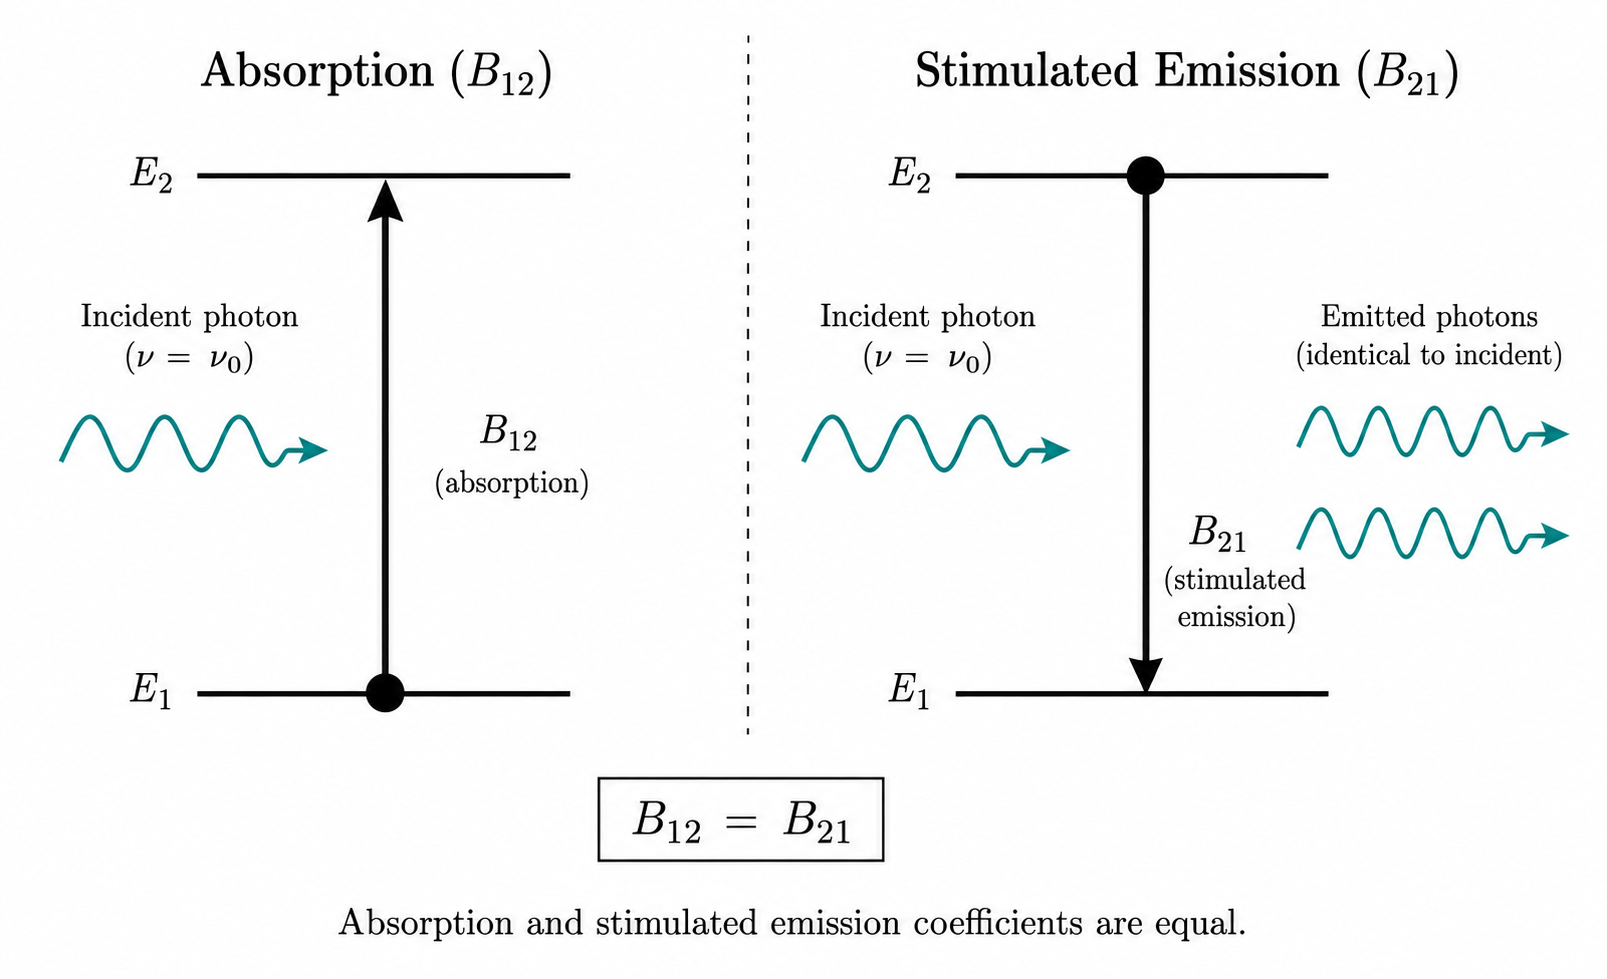
\includegraphics[width=0.6\textwidth]{Figures/Chapter 2/einstein_coefficients_symmetry.jpg}
    \caption{Einstein Coefficients Symmetry: Highlighting the fundamental equivalence ($B_{12} = B_{21}$) between the rates of upward absorption and downward stimulated emission.}
\end{figure}

With $B_{12} = B_{21} = B$, the equilibrium energy spectral density simplifies to:
\begin{equation*}
    \rho(\nu) = \frac{A}{B\left(e^{h\nu_0/(k_BT)} - 1\right)}
\end{equation*}

Comparing with the black-body formula:
\begin{equation*}
    \frac{A}{B\left(e^{h\nu_0/(k_BT)} - 1\right)} = \frac{8\pi h\nu_0^3}{c^3} \cdot \frac{1}{e^{h\nu_0/(k_BT)} - 1}
\end{equation*}

The temperature-dependent exponential factors perfectly cancel from both sides, leaving:
\begin{equation*}
    \frac{A}{B} = \frac{8\pi h\nu_0^3}{c^3}
\end{equation*}

Using the in-medium speed of light $c = \lambda\nu_0$, we substitute $c^3 = \lambda^3\,\nu_0^3$. Along with $A = 1/\tau_{sp}$:
\begin{equation*}
    \frac{1}{B\,\tau_{sp}} = \frac{8\pi h\nu_0^3}{c^3} = \frac{8\pi h\nu_0^3}{\lambda^3\nu_0^3} = \frac{8\pi h}{\lambda^3}
\end{equation*}

Inverting and dividing by $\tau_{sp}$ fully isolates $B$:
\begin{keyresult}
\begin{equation}
    B = B_{12} = B_{21} = \frac{\lambda^3}{8\pi h\,\tau_{sp}}
\end{equation}
\end{keyresult}

And the spontaneous emission rate is determined by the same chain:
\begin{keyresult}
\begin{equation}
    A = \frac{1}{\tau_{sp}} = \frac{8\pi h}{\lambda^3}\,B
\end{equation}
\end{keyresult}

These are the Einstein coefficients. The $A$ coefficient governs how quickly atoms spontaneously release energy from $E_2$; the $B$ coefficient (which is the same for absorption and stimulated emission) governs how strongly the atom responds to an external photon field.

\begin{keyinsight}[Symmetry of Absorption and Stimulated Emission]
Just as the $A$ coefficient defines the spontaneous lifetime $\tau_{sp} = 1/A$, the $B$ coefficient defines the \textbf{field-driven lifetimes} corresponding to absorption and stimulated emission against an applied photon field $\rho(\nu)$:
\begin{equation*}
    \tau_{\text{abs}} = \frac{1}{B_{12}\,\rho(\nu)} = \frac{1}{B\,\rho(\nu)}
    \qquad \text{and} \qquad
    \tau_{\text{stim}} = \frac{1}{B_{21}\,\rho(\nu)} = \frac{1}{B\,\rho(\nu)}
\end{equation*}
At the level of a single atom, the mathematical equality $B_{12} = B_{21}$ guarantees that $\tau_{\text{abs}} = \tau_{\text{stim}}$. The atom is perfectly agnostic: its inherent waiting time to absorb a photon from $E_1$ is identically equal to its waiting time to be stimulated down from $E_2$ by that same field. 
\end{keyinsight}

\subsection{The Limitation of the Einstein Model}

We now have the exact equations governing the transition rates between our energy levels. However, if we tried to immediately use these equations to calculate how a real optical beam's intensity grows or decays, our calculations would fail.

The problem lies in \textbf{broadening}. The Einstein model, as derived above, treats the atomic transition as an infinitely sharp occurrence—assuming that atoms only ever interact with light at the mathematically perfect resonance frequency $\nu_0$. 

In reality, as we learned from the classical model, light-matter interactions are smeared across a frequency band, governed by the line shape function $g_{\nu_0}(\nu)$. Because the Einstein model lacks a $g_{\nu_0}(\nu)$ term in its rate equations, it is physically incomplete. Before we can step back to the macroscopic scale to compute real optical intensities or gain, we must first explicitly correct our model so it distributes its interactions over a realistic frequency spectrum.

\section{Modification of the Einstein Model}

\subsection{The Physical Motivation: Uncertainty and Energy Level Spread}

In the classical oscillator model (Chapter 1), we explained line broadening phenomenologically through the damping friction $\eta$. How does broadening emerge in the quantum atomic model naturally, if an electron is simply jumping between two distinct, quantized energy levels? 

The fundamental quantum explanation is the \textbf{Heisenberg Uncertainty Principle}:
\begin{equation*}
    \Delta E \cdot \Delta t \gtrsim \hbar
\end{equation*}

If an atom spends a finite, statistically predictable lifetime $\Delta t$ in the excited state $E_2$ before decaying, its exact energy while stored in that state cannot be known with infinite precision. There is an inherent, inescapable spread $\Delta E$ in its energy level. 

Because the energy level is "smeared" by $\Delta E$, the energy required to bridge the transition is no longer a perfectly sharp single value. According to $E = h\nu$, this energy uncertainty translates directly into a frequency uncertainty:
\begin{equation*}
    \Delta\nu \approx \frac{\Delta E}{h}
\end{equation*}

This natural energy smearing is the precise quantum origin of the line shape function. The atom no longer mandates a photon of exactly the central resonance frequency. Instead, it can interact with any incoming photon of frequency $\nu$ that falls within the "blurred" energy band $\Delta\nu$ around the center.

To formalise this statistically, we define:
\begin{itemize}
    \item $h\nu_0 \equiv E_2 - E_1$: The energy difference between the exact geometric centres of the two energy levels. This defines the \textbf{resonance frequency} $\nu_0$, where the probability of interaction is strictly maximum.
    \item $h\nu$: The energy of an arbitrary incoming photon. If $\nu$ is close to $\nu_0$, the photon can successfully bridge the gap by leveraging the atom's energy uncertainty.
\end{itemize}

The statistical probability that an incoming photon of frequency $\nu$ successfully triggers a transition drops off the further $\nu$ drifts from the exact centre $\nu_0$. This probability distribution is exactly what the line shape function, $g_{\nu_0}(\nu)$, mathematically maps!

\begin{figure}[H]
    \centering
    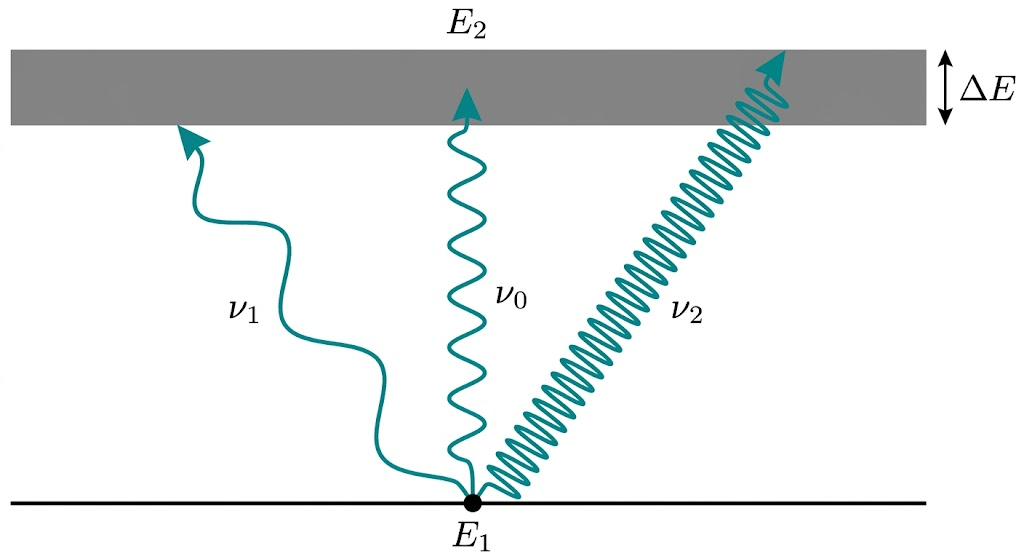
\includegraphics[width=0.6\textwidth]{Figures/Chapter 2/heisenberg_broadening.jpg}
    \caption{Heisenberg Uncertainty and Broadening: Quantum uncertainty dictates that the upper energy level is not perfectly sharp, creating a blurred energy band ($\Delta E$) and consequently a spread in acceptable transition frequencies ($\Delta\nu$) centered strictly around $\nu_0$.}
\end{figure}

\subsection{Incorporating the Line Shape Function into the Rate Equations}

To fix our theoretical gap, we must distribute the interaction probability across the physical frequency spectrum. We do this by redefining the transition probabilities for an infinitesimal frequency slice $d\nu$, multiplying by the line shape function $g_{\nu_0}(\nu)\,d\nu$.

The overall macroscopic transition rate is therefore the integral over all interaction frequencies:
\begin{align*}
    \left.\frac{dN_2}{dt}\right|_{sp} &= - \int_0^\infty A\,N_2\,g_{\nu_0}(\nu)\,d\nu \\[8pt]
    \left.\frac{dN_2}{dt}\right|_{abs} &= \int_0^\infty B\,N_1\,\rho(\nu)\,g_{\nu_0}(\nu)\,d\nu \\[8pt]
    \left.\frac{dN_2}{dt}\right|_{stim} &= - \int_0^\infty B\,N_2\,\rho(\nu)\,g_{\nu_0}(\nu)\,d\nu
\end{align*}

Notice a mathematical sanity check on the spontaneous emission integral. Because it does not depend on the external field $\rho(\nu)$, we can pull the constants out and use the normalisation $\int_0^\infty g_{\nu_0}(\nu)\,d\nu = 1$ directly. The integral instantly recovers the original unbroadened macroscopic rate $-A\,N_2 = -N_2/\tau_{sp}$, exactly as Einstein wrote it. The modification does not change spontaneous emission—it only reshapes how the atom couples to the incoming field.

\subsection{Evaluating the Integral: Narrow vs. Wide Spectral Sources}

The practical question is how to actually evaluate the integral $\int_0^\infty \rho(\nu)\,g_{\nu_0}(\nu)\,d\nu$ that appears in both the absorption and stimulated emission rates. The answer depends critically on the spectral shape of the driving field $\rho(\nu)$.

\begin{figure}[H]
    \centering
    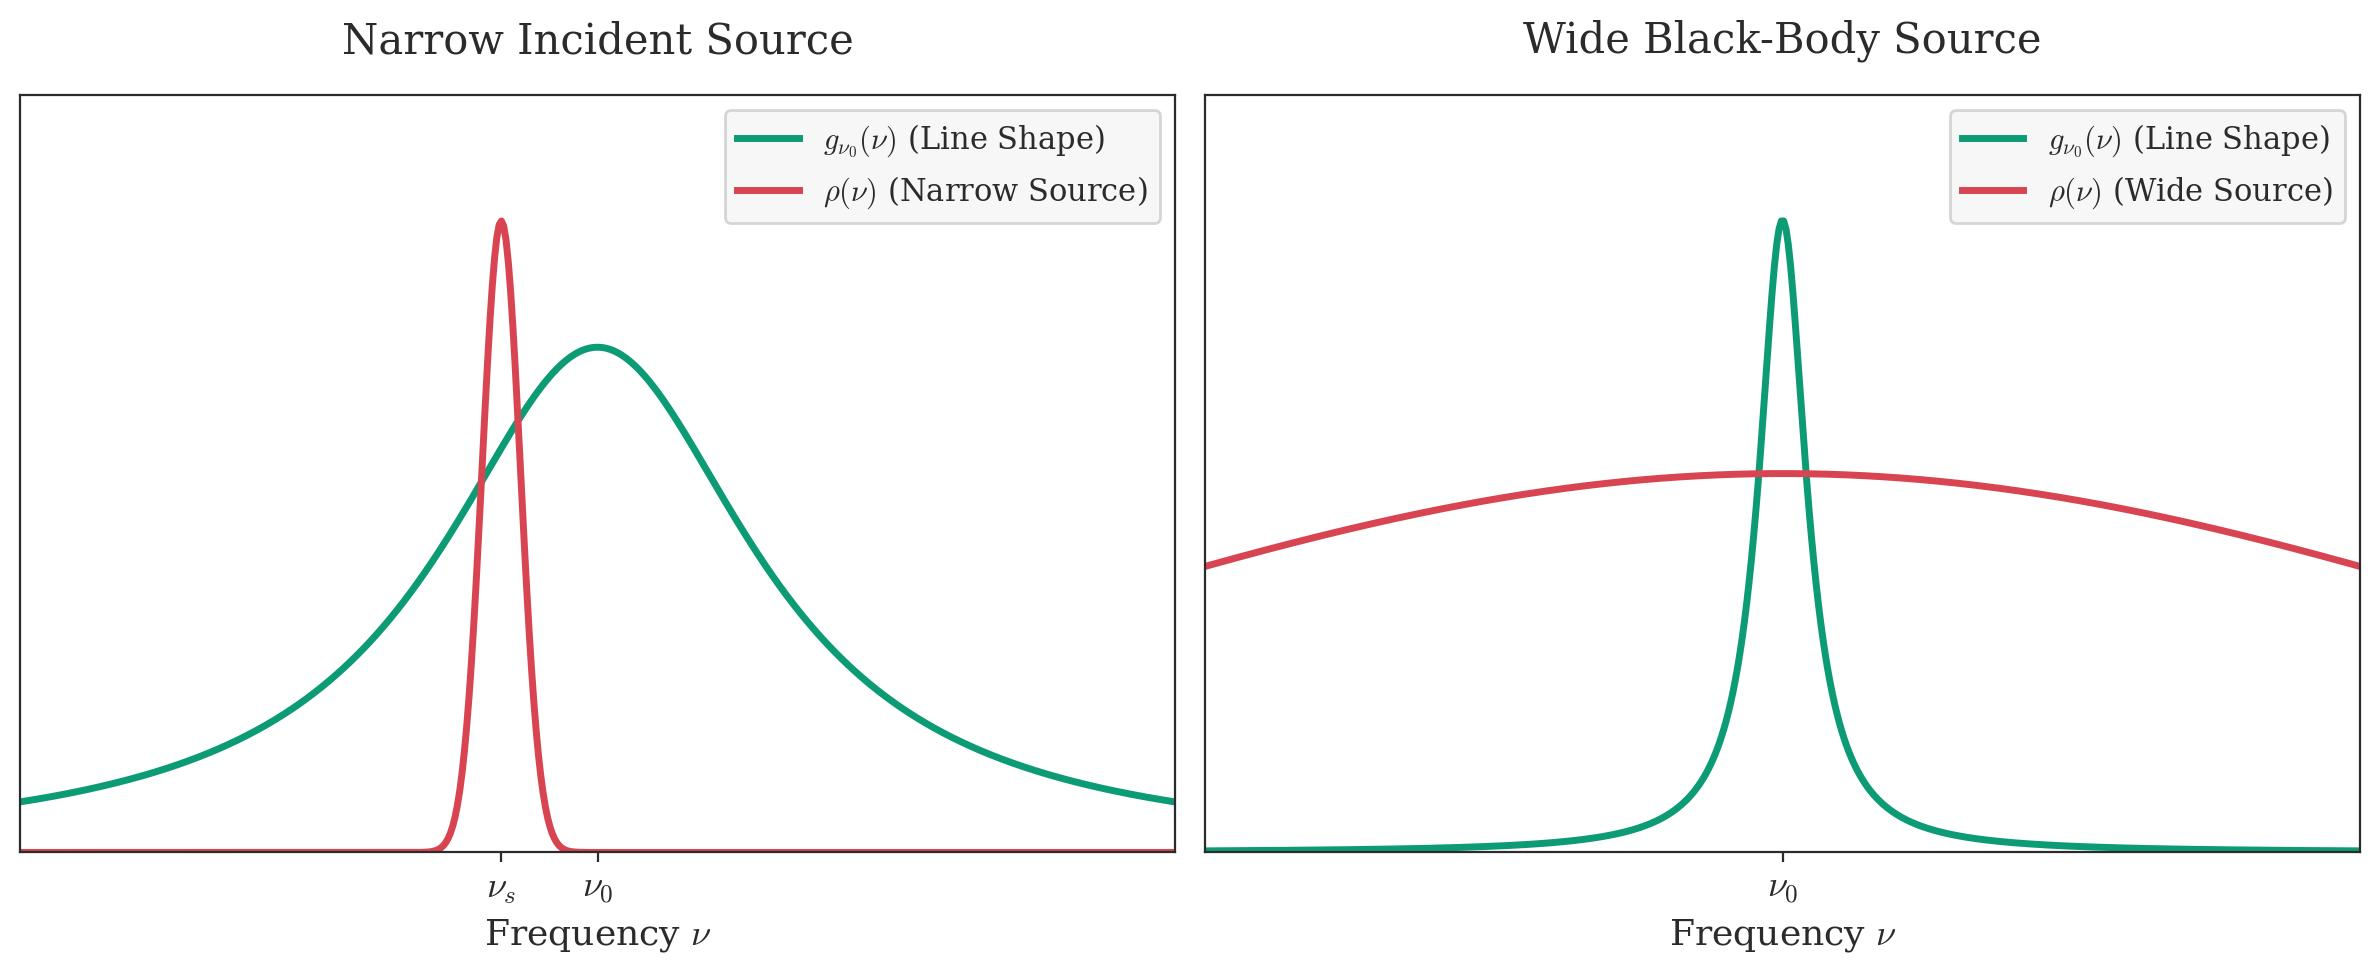
\includegraphics[width=0.85\textwidth]{Figures/Chapter 2/narrow_vs_wide_source.jpg}
    \caption{Spectral Overlap Regimes: (Left) A narrow laser source interacts strictly at its specific incident frequency $\nu_s$. (Right) A wide thermal black-body source sweeps broadly across the atom, experiencing the entire line shape simultaneously.}
\end{figure}

The evaluation splits into two extreme, mutually exclusive physical regimes:

\begin{itemize}
    \item \textbf{Case 1: The Narrow Light Source (e.g., a Laser).} 
    If the incident light is highly monochromatic (like a coherent laser), its energy density is razor-thin compared to the atom's acceptance line shape. We geometrically model this field as a Dirac delta function centered at the laser's frequency $\nu_s$: $\rho(\nu) \simeq \rho_\nu\,\delta(\nu - \nu_s)$. Here, $\rho_\nu$ is a scaling constant representing the \textbf{total integrated energy density} of the laser beam.
    
    Applying this to both the absorption and stimulated emission integrals, the delta function cleanly samples the line shape at exactly the laser's frequency $\nu_s$:
    \begin{align*}
        \left.\frac{dN_2}{dt}\right|_{abs} &= B\,N_1 \int_0^\infty \rho_\nu\,\delta(\nu - \nu_s)\, g_{\nu_0}(\nu)\,d\nu = B\,N_1\,\rho_\nu\, g_{\nu_0}(\nu_s) \\[8pt]
        \left.\frac{dN_2}{dt}\right|_{stim} &= -B\,N_2 \int_0^\infty \rho_\nu\,\delta(\nu - \nu_s)\, g_{\nu_0}(\nu)\,d\nu = -B\,N_2\,\rho_\nu\, g_{\nu_0}(\nu_s)
    \end{align*}
    Both rates are controlled by the exact same factor $\rho_\nu\,g_{\nu_0}(\nu_s)$—the atom's acceptance probability evaluated at the laser's specific driving frequency. The only difference between them is the population reservoir they draw from ($N_1$ for absorption, $N_2$ for stimulated emission).

    \item \textbf{Case 2: The Wide Black-Body Source (Thermal Equilibrium).} 
    Conversely, if the atom is bathed in a broad thermal source (like a hot cavity), the incident energy density $\rho(\nu)$ is incredibly wide and flat. Relative to the sharp atomic transition $g_{\nu_0}(\nu)$, $\rho(\nu)$ is effectively a slowly varying constant. 
    
    Because it barely changes over the interaction bandwidth, we can safely pull $\rho(\nu)$ outside the integral entirely:
    \begin{equation*}
        \int_0^\infty \rho(\nu) g_{\nu_0}(\nu)\,d\nu \approx \rho(\nu) \int_0^\infty g_{\nu_0}(\nu)\,d\nu = \rho(\nu) \cdot (1) = \rho(\nu)
    \end{equation*}
    By doing so, the line shape function disappears entirely! Both rates perfectly collapse back to Einstein's original unbroadened formulas: $+B\,N_1\,\rho(\nu)$ for absorption and $-B\,N_2\,\rho(\nu)$ for stimulated emission — exactly as he first derived them.
\end{itemize}

What this mathematical split reveals is that the atom acts as a natural filter for the incoming light. If you bathe the atom in a broad, noisy thermal spectrum (Case 2), the line shape effectively vanishes, and we perfectly recover Einstein's original model. But if you drive the atom with a sharp, coherent laser (Case 1), the transition rate becomes fiercely dependent on exactly how well your laser frequency $\nu_s$ aligns with the atom's internal probability curve $g_{\nu_0}(\nu_s)$. 

Because our ultimate goal is to engineer coherent lasers and optical amplifiers, we will discard the broad thermal model from this point forward. The remainder of our derivations will operate exclusively in the narrow-source laser regime.

\subsection{Bridging Energy Density to Optical Intensity}

In our laser-regime derivations, we successfully packaged the driving field into the integrated constant $\rho_\nu\, [\text{J/m}^3]$—the total physical electromagnetic energy stored within a unit volume of our material. However, energy density is a fundamentally static, locked-in-a-box concept. 

To actively engineer a real optical amplifier, we do not just care about stored energy; we care about the \textbf{optical intensity} $I_\nu$ of a travelling wave. We need to know whether the physical power continuously streaming across our crystal is amplifying or attenuating. 

To link this static energy volume to a travelling intensity, consider a small material slab of cross-sectional area $A$ and thickness $\Delta z$. The total electromagnetic energy stored inside the slab is $\rho_\nu \cdot A \cdot \Delta z$. Since photons travel through the medium at the group velocity $V_g$, the time taken to traverse the slab is $\Delta t = \Delta z / V_g$, so the power streaming through area $A$ is:

\begin{equation*}
    \text{Power} = \frac{\text{Energy}}{\Delta t} = \frac{\rho_\nu \cdot A \cdot \Delta z}{\Delta t} = \rho_\nu \cdot A \cdot V_g
\end{equation*}

Intensity is power per unit cross-sectional area, so dividing by $A$ immediately gives:
\begin{equation}
    I_\nu = \rho_\nu\,V_g
\end{equation}

In a standard non-dispersive medium, photons travel precisely at the speed of light in that medium, meaning the group velocity is simply $V_g = c$. Therefore, navigating from intensity back to energy density mathematically reduces to:
\begin{keyresult}
\begin{equation*}
    \rho_\nu = \frac{I_\nu}{c}
\end{equation*}
\end{keyresult}

\subsection{The Photon Flux Density \texorpdfstring{$\Phi$}{Phi}}

While calculating macroscopic power using the travelling intensity $I_\nu$ is practically useful for engineering, we must remember that interactions at the atomic level are purely discrete. An atom does not absorb a continuous stream of "power"; it only captures discrete, individual photons. Therefore, to rigorously model how frequently these microscopic energy transitions occur, we must physically translate our continuous wave intensity into a strict particle count—exactly how many individual photons traverse a single unit of cross-sectional area every second. We define this as the \textbf{photon flux density} $\Phi$.

\begin{keyresult}
\begin{equation}
    \Phi = \frac{\text{Number of incident photons}}{\text{sec} \cdot \text{m}^2}
\end{equation}
\end{keyresult}

Because each distinct photon carries an exact quantum of energy $E = h\nu$, the macroscopic intensity $I_\nu$ is simply the photon flux multiplied by the energy of a single photon:
\begin{equation*}
    I_\nu = \Phi\,h\nu
\end{equation*}

This provides the final, complete mathematical bridge from our original abstract energy density $\rho_\nu$ all the way down to a discrete photon flux. Substituting this into our intensity relation gives:
\begin{equation*}
    \rho_\nu = \frac{I_\nu}{c} = \frac{h\nu}{c}\,\Phi
\end{equation*}

With this purely flux-based expression for the driving field, we are ready to assemble the final macroscopic rate equation. Recall from the narrow-source laser derivation that both the absorption and stimulated emission rates are fundamentally driven by the exact same field-coupling factor $B\,\rho_\nu\,g_{\nu_0}(\nu)$. Because the physics is identically symmetric, we can pick either process to perform our underlying algebra. Let's select the \textbf{stimulated emission} rate:
\begin{equation*}
    \left.\frac{dN_2}{dt}\right|_{stim} = -B\,N_2\,\rho_\nu\,g_{\nu_0}(\nu)
\end{equation*}

Substitute our flux-based $\rho_\nu$ alongside the Einstein in-medium $B$ coefficient $\left(B = \dfrac{\lambda^3}{8\pi h\,\tau_{sp}}\right)$ explicitly into this rate equation:
\begin{align*}
    \left.\frac{dN_2}{dt}\right|_{stim} &= -\left( \frac{\lambda^3}{8\pi h\,\tau_{sp}} \right) N_2 \left( \frac{h\nu}{c}\,\Phi \right) g_{\nu_0}(\nu)
\end{align*}

To systematically simplify this, we group the constants, cancel the Planck constant $h$, and substitute the standard in-medium speed of light identity $c = \lambda\nu$:
\begin{equation*}
    \left.\frac{dN_2}{dt}\right|_{stim} = -\frac{\lambda^3\,\nu\,h}{8\pi h\,\tau_{sp}\,c}\,N_2\,\Phi\,g_{\nu_0}(\nu) = -\frac{\lambda^3\,\nu}{8\pi\,\tau_{sp}\,(\lambda\nu)}\,N_2\,\Phi\,g_{\nu_0}(\nu) = -\frac{\lambda^2}{8\pi\,\tau_{sp}}\,N_2\,\Phi\,g_{\nu_0}(\nu)
\end{equation*}

Once the speed of light $c$ and the wave frequency $\nu$ cleanly cancel from the algebra, we are left with an elegantly compact mathematical multiplier attached to our photon flux $\Phi$. 

But why is this specific multiplier physically meaningful? Consider the dimensional analysis: our photon flux $\Phi$ is measured in \textit{photons per second per square meter} ($1/(\text{s}\cdot\text{m}^2)$). For the equation to correctly resolve into a transition rate (events per second), this new multiplier must possess the exact SI units of \textbf{area} ($\text{m}^2$). 

Physically, this multiplier represents the effective "target size" that an individual atom presents to the incoming photon beam. If an incident photon passes through this microscopic interaction area, it successfully triggers a transition. Because of this powerful geometrical interpretation, we formally identify this term as the \textbf{stimulated emission cross-section} $\sigma(\nu)$!

\begin{keyresult}
\begin{equation}
    \sigma(\nu) = \frac{\lambda^2}{8\pi\,\tau_{sp}}\,g_{\nu_0}(\nu)
\end{equation}
\end{keyresult}

Notice a critical structural distinction. The quantum Einstein cross-section differs from the classical oscillator cross-section $\left(\sigma_{classical} = \frac{3\lambda^2}{8\pi\tau_r}g(\nu)\right)$ by exactly a factor of 3. That factor of 3 is not accidental—our quantum derivation automatically accounted for the directional degeneracy of the photon polarisation states in 3D space, something the crude 1D classical spring model fundamentally cannot do. The Einstein expression is the correct one.

\subsection{The Master Rate Equations}

Because absorption and stimulated emission share the exact same physical coupling, applying our $\sigma(\nu)$ algebraic result to both reveals that they possess identically symmetric per-atom transition rates.

Combining these two field-driven rates with our spontaneous decay term, we can now assemble the final, master forms of all three macroscopic population rate equations acting on the excited state $N_2$:

\begin{align*}
    &\textbf{Spontaneous emission:} & \left.\frac{dN_2}{dt}\right|_{sp} &= -\frac{N_2}{\tau_{sp}} \\[8pt]
    &\textbf{Absorption:} & \left.\frac{dN_2}{dt}\right|_{abs} &= \sigma(\nu)\,\Phi\,N_1 \\[8pt]
    &\textbf{Stimulated emission:} & \left.\frac{dN_2}{dt}\right|_{stim} &= -\sigma(\nu)\,\Phi\,N_2
\end{align*}

Notice that exactly the same field-coupling factor, $\sigma(\nu)\,\Phi$, governs both field-driven interactions. Recall our earlier definition of the field-driven lifetimes. Because the transition cross-section completely encapsulates the interaction physics, we can now express the \textbf{absorption lifetime} $\tau_{abs}$ and \textbf{stimulated lifetime} $\tau_{stim}$ directly in terms of the driving photon flux:
\begin{equation*}
    \frac{1}{\tau_{abs}} = \frac{1}{\tau_{stim}} \equiv \sigma(\nu)\,\Phi
\end{equation*}

Because the laser field is equally effective at driving atoms upward as it is at driving them downward, the final outcome of the interaction is purely a numbers game. The net flow of optical power depends entirely on which population reservoir is larger. If the ground state holds more atoms ($N_1 > N_2$), those atoms act as a sink, and the material will net-absorb the beam. But if we can somehow artificially force more atoms into the excited state ($N_2 > N_1$), the material will net-amplify the incoming beam through stimulated emission.

\begin{figure}[H]
    \centering
    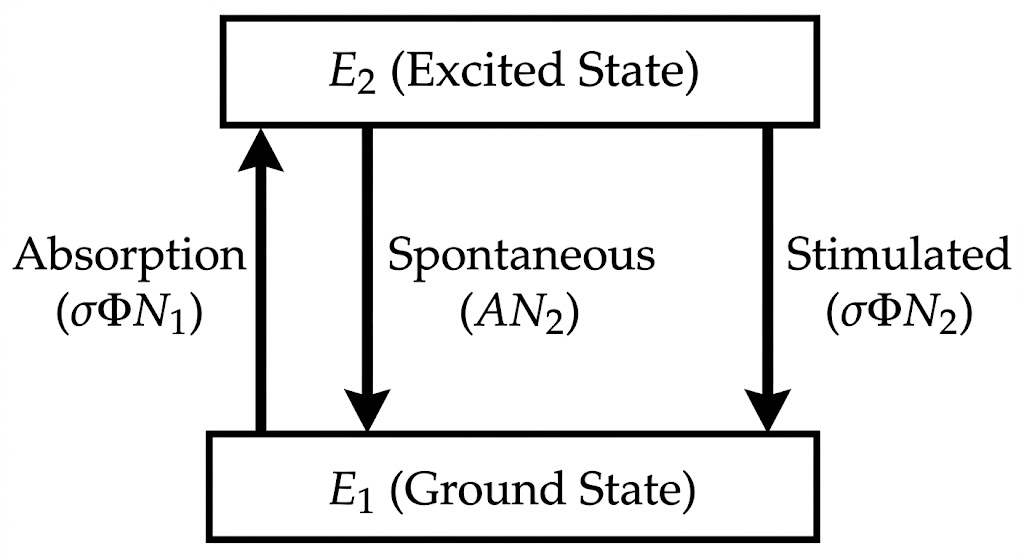
\includegraphics[width=0.6\textwidth]{Figures/Chapter 2/population_flows_summary.jpg}
    \caption{Summary of Population Flows: A consolidated overview of the three fundamental processes—absorption, spontaneous emission, and stimulated emission.}
\end{figure}

\begin{table}[H]
\centering
\begin{tabular}{@{}llll@{}}
\toprule
\textbf{Process} & \textbf{Rate coefficient} & \textbf{Direction of $N_2$} & \textbf{Requires external field?} \\
\midrule
Spontaneous emission & $A = 1/\tau_{sp}$ & Decreases (-) & No \\
Absorption & $\sigma(\nu)\Phi = 1/\tau_{abs}$ & Increases (+) & Yes \\
Stimulated emission & $\sigma(\nu)\Phi = 1/\tau_{stim}$ & Decreases (-) & Yes \\
\bottomrule
\end{tabular}
\end{table}

\section{Macroscopic Propagation: The Gain Coefficient}

We have successfully established how atomic populations act on an incident optical field entirely at the microscopic limit. But optical engineering is fundamentally continuous and macroscopic — we need to know what mathematically happens to a beam of light as it physically travels across a distance $z$ through a bulk semiconductor chunk. Does the beam amplify, or does it die out?

To answer this, we establish a simple one-dimensional control volume. Imagine an optical beam with cross-sectional $\text{Area}$ traveling along the $z$-axis. It enters a tiny slice of the material at position $z$, and exits at position $z + \Delta z$. The total volume of this physical slice is $V = \text{Area} \cdot \Delta z$.

Inside this bounded volume, the macroscopic beam interacts with the microscopic atomic populations. The beam loses photons when atoms jump to $E_2$ (absorption), and gains perfectly aligned "clone" photons when atoms are stimulated down to $E_1$ (stimulated emission). 

But wait, why isn't spontaneous emission included in this spatial equation? Because spontaneous emission ejects photons completely randomly across all directions in 3D space, the vast majority of those photons simply shoot out the sides of our control volume and escape. They do not join our strict $z$-axis beam path. Therefore, from the perspective of our perfectly directed traveling flux $\Phi(z)$, spontaneous emission is considered entirely lost.

Through simple particle accounting, the physical change in the number of travelling photons exiting the slice per second must perfectly equal the rate of new photons created by stimulated emission minus the rate of photons destroyed by absorption inside that volume:
\begin{equation*}
    \text{Area} \cdot \big(\Phi(z + \Delta z) - \Phi(z)\big) = \big(\sigma(\nu)\,\Phi\,N_2 - \sigma(\nu)\,\Phi\,N_1\big) \times (\text{Area} \cdot \Delta z)
\end{equation*}

We can immediately divide out the cross-sectional $\text{Area}$ from both sides. By isolating the terms and taking the mathematical limit as our slice thickness shrinks to zero ($\Delta z \to 0$), the discrete finite difference elegantly collapses into a continuous spatial differential equation:
\begin{align*}
    \frac{\Phi(z + \Delta z) - \Phi(z)}{\Delta z} &= \sigma(\nu)\,(N_2 - N_1)\,\Phi \\[8pt]
    \frac{d\Phi}{dz} &= \sigma(\nu)\,(N_2 - N_1)\,\Phi
\end{align*}

We can see that the spatial rate of change of the photon flux is directly proportional to the flux itself, scaled by a constant material factor. We formally group this material factor $\sigma(\nu)(N_2 - N_1)$ into a single macroscopic parameter called the \textbf{gain coefficient} $\gamma(\nu)$.

\begin{keyresult}
\begin{equation}
    \gamma(\nu) = \sigma(\nu)(N_2 - N_1)
\end{equation}
\end{keyresult}

Replacing this into our differential equation yields the beautiful, compact spatial propagation law:
\begin{equation*}
    \frac{d\Phi}{dz} = \gamma(\nu)\,\Phi
\end{equation*}

This is a classic first-order linear differential equation. If we assume the beam enters the material at $z=0$ with an initial flux $\Phi(0)$, solving the differential equation reveals a harsh, exponential spatial profile:
\begin{equation*}
    \Phi(z) = \Phi(0)\,e^{\gamma(\nu) z}
\end{equation*}

\begin{keyinsight}[The Possibility of Gain]
This singular exponential equation dictates the entire macroscopic fate of the optical beam. The physics is completely controlled by the algebraic sign of the gain coefficient $\gamma(\nu)$, driving two spectacularly distinct physical regimes:
\begin{itemize}
    \item \textbf{Case 1: Optical Loss.} Under normal thermodynamic conditions governed by Boltzmann statistics, the ground state is always significantly more populated than the excited state ($N_1 > N_2$). The term $(N_2 - N_1)$ is mathematically negative, making the gain coefficient $\gamma$ negative. The resulting profile $\Phi(z) = \Phi(0)e^{-|\gamma(\nu)| z}$ describes classic \textbf{exponential decay}. The bulk material acts as an optical absorber.
    
    \item \textbf{Case 2: Optical Amplification.} If we aggressively pump the material with external energy, we can artificially force more atoms into the higher energy state. When we cross the threshold of $N_2 > N_1$, we achieve a \textbf{population inversion}. The term $(N_2 - N_1)$ explicitly flips positive, making $\gamma$ positive. The resulting profile $\Phi(z) = \Phi(0)e^{+\gamma(\nu) z}$ now describes explosive \textbf{exponential growth}. The material has successfully become an optical amplifier, providing the very "gain" necessary to build a laser!
\end{itemize}
\end{keyinsight}
